\section{Residue Number Systems}
\label{sec:rns}
In BGV, BFV and CKKS the ciphertext modulus $Q$ is large --- much larger than a computer word (typically 64 bits on modern computers). Multi-precision arithmetic is known to be slow due to its serial nature, so implementations avoid it by using a \gls{rns}, which represents large numbers as a set of smaller, independent residues. RNS variants of BGV, BFV and CKKS are the standard in practice; OpenFHE, for example, only supports the RNS versions of these schemes.

\begin{definition}[Canonical Form]
    We are interested in polynomials in the ring $R_Q = \mathbb{Z}_Q[X]/(X^N+1)$ with degree (up to) $N - 1$ and coefficients in $[-Q/2, Q/2)$ (centered modulo representation), and different ways to represent this polynomial. The canonical form \eqref{form:canonical} of such a polynomial $a$ is the form everyone is familiar with.
    \begin{equation}
        \label{form:canonical}
        a = c_0 + c_1X + \cdots + c_{N-1}X^{N-1} = \sum_{i=0}^{N-1} c_iX^i
    \end{equation}
\end{definition}

\begin{definition}[Coefficient Form]
    As polynomials have a well-known/predictable structure, we can omit the redundant $X$ variable and represent $a\in R_Q$ uniquely by its coefficients. I will refer to (only) this representation \eqref{form:coefficient} as the \emph{coefficient} form.  
    \begin{equation}
        \label{form:coefficient}
        a = (c_0, c_1, \dots, c_{N-1})
    \end{equation}
\end{definition}

Let $Q = q_0\dots q_{k-1}$ with $\gcd(q_i, q_j) = 1 \;\forall\; i\not= j$, so that the \gls{crt} allows decomposition into smaller residues. If $\max_i\{q_i\}$ fits in a computer word then we can use \gls{crt} on the coefficients of a polynomial to work exclusively with integers that fit inside a computer word.

%%
%% COEFFICIENT FORMAT
\begin{definition}[CRT Form]
    Given a polynomial $a \in R_Q$ where $Q = q_0q_1\dots q_{k-1}$ is chosen as a product of $k$ small primes (small meaning they each fit inside a computer register), each coefficient $c_i$ is uniquely represented by its $k$ residues via the Chinese Remainder Theorem. Then the \emph{CRT form} of $a$ \eqref{form:crt} is a collection of smaller polynomials ($\bmod{q_i}$) called \textit{towers}, \textit{residues} or \textit{limbs}.

    \begin{equation}
    \label{form:crt}
    % \ifnotes
        \begin{pmatrix}
            a\mod q_0 \\
            a\mod q_1 \\
            \vdots \\
            a\mod q_{k-1}
        \end{pmatrix}
        =
    % \fi
    \begin{pmatrix}
        c_0 \bmod{q_0} & c_1 \bmod{q_0} & \dots & c_{N-1}\bmod{q_0} \\
        c_0 \bmod{q_1} & c_1 \bmod{q_1} & \dots & c_{N-1}\bmod{q_1} \\
        \vdots & \vdots & \ddots & \vdots \\
        c_0 \bmod{q_{k-1}} & c_1 \bmod{q_{k-1}} & \dots & c_{N-1}\bmod{q_{k-1}}
    \end{pmatrix}
    \end{equation}
\end{definition}

Addition and subtraction of two polynomials in $R_Q$ is equivalent to element-wise addition/subtraction of their CRT forms (modulo $q_i$). As each element fits within a computer word, no carries propagate between them, and all pairs of elements can be added or subtracted in parallel.

% \noindent Clearly, the $i$-th column of \eqref{form:crt} is a CRT problem for $c_i$, so converting between this and the canonical form $\sum_{i=0}^{N-1}c_iX^i$ or vector form $(c_0,c_1,\dots, c_{N-1})$ is easy. \textcolor{red}{\textbf{Note that confusingly ``coefficient format'' is used in OpenFHE about this form specifically, NOT the ``vector'' form which is normally used in the literature... kjært barn har mange navn..}}

\begin{remark}
    \textcolor{red}{Rather confusingly, OpenFHE calls this form \emph{Coefficient} format. Both RNS forms are represented by an \texttt{DCRTPoly} object, so a polynomial in CRT form is represented by a \texttt{DCRTPoly} object in \texttt{Format::Coefficient} mode.}
    \begin{figure}[ht!]
        \centering
        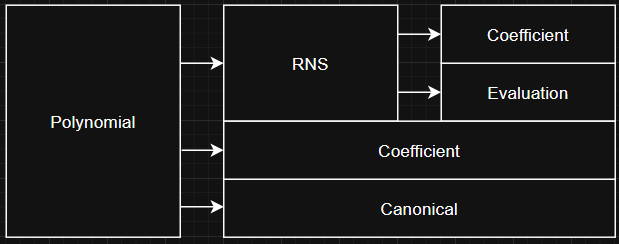
\includegraphics[width=0.4\linewidth]{Figures/representations.png}
    \end{figure}
\end{remark}

%%
%% EVALUATION FORMAT
\subsection{Number Theoretic Transform}
% Maybe more details in appendix?
The \gls{ntt} converts a negacyclic convolution in the coefficient domain into point-wise multiplication in the NTT domain --- and multiplication in $R_{q_i}$ is exactly such a convolution of the coefficient vectors. Applying the \gls{ntt} to each residue (row) of the CRT form \eqref{form:crt} therefore makes polynomial multiplication element-wise as well. The negacyclic \gls{ntt} of size $N$ requires each modulus to satisfy $q_i \equiv 1 \pmod{2N}$, which constrains the choice of RNS primes.

\begin{definition}[Double CRT/NTT/Evaluation Form]
    By applying the \gls{ntt} to the CRT form \eqref{form:crt} we gain the ability to perform polynomial multiplication in parallel, without losing the ability to perform addition/subtraction in parallel.
    
    \begin{equation}
        \label{form:eval}
        \begin{pmatrix}
            \ntt{a\bmod q_0} \\
            \ntt{a\bmod q_1} \\
            \vdots \\
            \ntt{a\bmod q_{k-1}}
        \end{pmatrix}
        =
        \begin{pmatrix}
            \hat{a}_{0,0} & \hat{a}_{0,1} & \dots & \hat{a}_{0,N-1} \\
            \hat{a}_{1,0} & \hat{a}_{1,1} & \dots & \hat{a}_{1,N-1} \\
            \vdots & \vdots & \ddots & \vdots \\
            \hat{a}_{k-1,0} & \hat{a}_{k-1,1} & \dots & \hat{a}_{k-1,N-1}
        \end{pmatrix}
    \end{equation}
    
\end{definition}

%%
%% CLOSING REMARKS
The evaluation form \eqref{form:eval} is the preferred form, as it supports parallel addition, subtraction and multiplication, but it still does not natively support \textit{all} necessary operations. Because switching between canonical/vector, CRT and NTT mode is relatively expensive --- requiring (inverse) CRTs and NTTs --- much of the relevant literature \cite{cryptoeprint:2012/099, cryptoeprint:2016/510, cryptoeprint:2018/117, cryptoeprint:2021/204} improves upon existing functions by finding new approaches and approximations that limit the number of format-switches required. 
\begin{equation*}
    \raisebox{0.3ex}{\text{ Coefficient }}
    \overset{\text{\tiny CRT}}{\underset{\text{\tiny iCRT}}{\overset{\longrightarrow}{\longleftarrow}}}
    \raisebox{0.3ex}{\text{ CRT }}
    \overset{\text{\tiny NTT}}{\underset{\text{\tiny iNTT}}{\overset{\longrightarrow}{\longleftarrow}}}
    \raisebox{0.3ex}{\text{ Evaluation (DCRT) }}
\end{equation*}

% Switching between formats is expensive so we try to stay in evaluation mode for as long as possible, only switching to coefficient/CRT form when absolutely required.




\subsection{RNS Base Conversion}
\label{sec:rns-base-conversion}
Several ciphertext maintenance operations --- most importantly the key-switching procedures of the next section --- temporarily extend the ciphertext modulus $Q$ by an auxiliary modulus $P$ and later scale back down. In RNS this corresponds to moving a polynomial between different RNS bases. I start by introducing some terminology.

\begin{definition}[RNS Basis.] 
    Given a large modulus $Q = \prod_{i=0}^{k-1} q_i$ composed of pairwise coprime factors, we define the \textit{RNS basis} $\mathcal{B}_Q = \{q_0, q_1, \dots, q_{k-1}\}$ as the set of RNS moduli used in the RNS/CRT representation \eqref{form:crt}.
\end{definition}

%%
%% BASE EXTENSION (NAIVE)
\iftrue{ % AI Written: Claude Fable
    % \color{purple}
    \begin{definition}[Base conversion]
        Let $\mathcal{B}_Q = \{q_0,\dots,q_{k-1}\}$ and
        $\mathcal{B} = \{b_0,\dots,b_{\ell-1}\}$ be RNS bases with
        $\gcd(Q, B) = 1$, where $B = \prod_{j} b_j$. Base conversion is
        the map that takes the representation of $x$ in $\mathcal{B}_Q$
        to the representation of $[x]_Q$ in $\mathcal{B}$, i.e.
        \[
            \big([x]_{q_0}, \dots, [x]_{q_{k-1}}\big)
            \;\longmapsto\;
            \big([x]_{b_0}, \dots, [x]_{b_{\ell-1}}\big).
        \]
        When the residues in $\mathcal{B}$ are appended to those in $\mathcal{B}_Q$, so that $x$ becomes represented in the \textit{extended} basis $\mathcal{B}_Q \cup \mathcal{B}$ for the modulus $QB$, the operation is also referred to as \emph{base extension}.
    \end{definition}
}\fi

% \begin{definition}[Base Extension.]
%     Special case of base conversion where we convert from $\mathcal{B}_Q \longmapsto \mathcal{B}_{QP}$. Note $\mathcal{B}_{QP} = \mathcal{B}_{Q} \cup \mathcal{B}_{P}$ and $P = \prod_i p_i$ etc. 
% \end{definition}

\begin{remark}
    Extend mod notation for RNS polynomials: $[a]_{\mathcal{B}_Q} = ([a]_{q_0}, \dots, [a]_{q_{k-1}})$ for the basis $\mathcal{B}_Q = \{q_i\}_{i=0}^{k-1}$ means $a$ must be in RNS form (\textcolor{red}{TODO: distinguish CRT vs NTT mode... maybe $[a]^\mathsf{NTT}_{\mathcal{B}_Q}$?})
\end{remark}

The naive approach to base conversion reconstructs $a$ from its residues via the \gls{crt} and then reduces the result modulo each modulus of the new basis. This reintroduces the multi-precision arithmetic that RNS was meant to avoid. A cheap but approximate alternative exists, described next.

%%%
%%% Base Extension
%%%
% \begin{algorithm}[ht!]
% \caption{Base Extension}
% \label{alg:base_extension}
% \begin{algorithmic}[1]
%     \Require $[a]_{\mathcal{B}_Q}^\mathsf{NTT}$ and a basis $\mathcal{B}_P$
%     \Ensure $[a]_{\mathcal{B}_{QP}}^\mathsf{NTT}$
%     \State Initialize an empty array $a_{P}$ of size $|\mathcal{B}_P|$
%     \Comment{Holds the $P$-towers}
%     \State $a_{\mathsf{coeffs}} := \mathsf{Inverse CRT}(\mathsf{Inverse NTT}(a))$
%     \Comment{Convert to coefficient form}
%     \For{$p_i \in \mathcal{B}_P$}
%         \State $a_{p_i} := a_{\mathsf{coeffs}} \pmod{p_i}$ \Comment{Find $p_i$-tower}
%         \State Append $\mathsf{NTT}(a_{p_i})$ to $a_{P}$
%     \EndFor
%     \State\Return $a \cup a_{P}$
% \end{algorithmic}
% \end{algorithm}

% \begin{enumerate}
%     \item Convert to RNS-coefficient mode, then convert to canonical/coefficient form
%     \item Find the residues/towers $\bmod{p_i}$ for $\mathcal{B}_P$
%     \item Apply NTT to each residue ($\bmod{p_i}$)
%     \item Append the NTT'd $P$-towers to the original $Q$-towers
% \end{enumerate}

\subsubsection{Fast Base Conversion}
Fast base conversion, introduced by \cite{cryptoeprint:2016/510}, performs the conversion directly on the residues (in CRT mode), avoiding the CRT reconstruction and multi-precision integers entirely. The price is approximation: \eqref{eq:fastbconv} produces not $x$ but $x + \alpha_x Q$ for some integer $\alpha_x \in [0, k)$, as computing the exact overflow $\alpha_x$ would require costly operations in RNS.

\begin{equation}
    \label{eq:fastbconv}
    \mathsf{FastBConv}(x, \mathcal{B}_Q, \mathcal{B}) = \left(\left[\sum_{i=0}^{k-1}\left[x_i\left(\frac{Q}{q_i}\right)^{-1}\right]_{q_i} \times \frac{Q}{q_i}\right]_b\right)_{b\in \mathcal{B}}
\end{equation}


\subsubsection{Fast Base Extension}
We can use \eqref{eq:fastbconv} as a subroutine in base extension: only the new residues $\mathcal{B}_Q \longmapsto \mathcal{B}_P$ need to be calculated, and since $\mathcal{B}_{QP} = \mathcal{B}_Q\cup \mathcal{B}_P$ the original residues are simply kept.

%%%
%%% Fast Base Extension
%%%
\begin{algorithm}[ht!]
\caption{Fast Base Extension}
\label{alg:fast_base_extension}
\begin{algorithmic}[1]
    \Require $[a]_{\mathcal{B}_Q}$ and a basis $\mathcal{B}_P$
    \Ensure $[a + \epsilon]_{\mathcal{B}_{QP}}$, where $\epsilon = \alpha_aQ$ for some $\alpha_a\in[0, k)$
    \State $a_{Q} := \mathsf{Inverse NTT}(a)$
    \Comment{Convert to CRT form}
    \State $a_{P} := \mathsf{FastBConv}(a_Q, \mathcal{B}_Q, \mathcal{B}_P)$
    \State\Return $a \cup \mathsf{NTT}(a_{P})$
\end{algorithmic}
\end{algorithm}

Notably, \eqref{eq:fastbconv} is approximate as a \textit{conversion} but exact as an \textit{extension}: the extended residue vector over $\mathcal{B}_Q\cup\mathcal{B}_P$ is an exact RNS representation of the lifted integer $x' = [x]_Q + \alpha_x Q \in \mathbb{Z}_{QP}$, since $\alpha_x Q \equiv 0 \pmod{q_i}$ keeps the original (reused) $Q$-residues consistent with $x'$. The RNS schemes are designed to tolerate this overflow, which is removed --- or shrunk to the small $\alpha_x$ --- by a subsequent division during mod down.

% \iftrue{
%     \color{red}
%     3. The fast variant is approximate as a conversion but exact as an extension. This is the deepest justification, and it's worth a remark in your text. FastBConv doesn't compute [x]Q mod bj[x]_Q \bmod b_j
%     [x]Q​modbj​; it computes (x+uQ) mod bj(x + uQ) \bmod b_j
%     (x+uQ)modbj​ for some small overflow uu
%     u. Viewed as a conversion, that's an error. But viewed as an extension, the combined residue vector over BQ∪B\mathcal{B}_Q \cup \mathcal{B}
%     BQ​∪B is a perfectly consistent, exact RNS representation of the single lifted integer x′=[x]Q+uQ∈ZQBx' = [x]_Q + uQ \in \mathbb{Z}_{QB}
%     x′=[x]Q​+uQ∈ZQB​ — the original residues still agree with x′x'
%     x′ modulo each qiq_i
%     qi​, since uQuQ
%     uQ vanishes there. The RNS-variant schemes are designed around exactly this: they tolerate carrying x′x'
%     x′ instead of xx
%     x because a subsequent division by QQ
%     Q shrinks uQuQ
%     uQ to the small quantity uu
%     u, or because a Shenoy–Kumaresan-style correction (your FastBConvEx) removes it using one extra modulus. So "extension" isn't just the more common use case — it's the semantics under which the fast algorithm is actually correct.
% }\fi

\begin{remark}
    The factors $[(\frac{Q}{q_i})^{-1}]_{q_i}$ and $\frac{Q}{q_i}$ can be pre-calculated and stored in memory (will be discussed in \autoref{sec:impl:hps}).
\end{remark}


% This conversion is relatively fast. This is because the sum should ideally be
% reduced modulo q in order to provide the exact value x; instead, (2) provides
% x + αxq for some integer αx ∈ [0, k − 1]. Computing αx requires costly operations
% in RNS. So this step is by-passed, at the cost of an approximate result.
% FastBconv naturally extends to polynomials of R by applying it coefficient-
% wise.

% , which requires no such conversion but does result in some noise. \eqref{eq:fastbconv} converts $x$ from base $Q$ to base $B$. Using this we can convert the residues of $a \in R_Q$ to residues in $R_P$ and simply add the towers to \eqref{form:eval}.

\subsubsection{Modulus Switching}
In RNS, modulus switching --- also referred to as \textit{mod down} --- from $Q$ to $Q' = Q/q_{k-1}$ amounts to \textit{dropping the last limb} with a small correction, computed limb-wise without CRT reconstruction:
\begin{equation}
    \label{eq:rns-modswitch}
    [c']_{q_i} = \left[q_{k-1}^{-1}\left(c - \delta\right)\right]_{q_i}, \quad 0 \leq i < k-1,
\end{equation}
where $\delta \equiv c \pmod{q_{k-1}}$ and, for BGV, $\delta \equiv 0 \pmod{t}$ so that decryption correctness is maintained. The noise shrinks by a factor $q_{k-1}$, matching the classical modulus switch.

\subsubsection{Approximate Mod Down $QP \to Q$}
The reverse operation, switching from the extended modulus $QP$ back down to $Q$, uses \eqref{eq:fastbconv} to convert the $P$-part back to $\mathcal{B}_Q$ before dividing by $P$ \autocite{cryptoeprint:2012/099, cryptoeprint:2018/117}:
\begin{equation}
    \label{eq:approxmoddown}
    \mathsf{ModDown}(x) = \left[P^{-1}\left(x - \mathsf{FastBConv}([x]_{\mathcal{B}_P}, \mathcal{B}_P, \mathcal{B}_Q)\right)\right]_{\mathcal{B}_Q}
\end{equation}
For BGV the converted term must additionally be corrected modulo $t$ to preserve the plaintext \cite{cryptoeprint:2021/204}. This operation also corrects the fast base conversion error: the conversion overflow $\alpha P$ is divided by $P$, shrinking it to the small additive term $\alpha$ --- which is why the approximation in \eqref{eq:fastbconv} is tolerable.
